\documentclass[a4paper,11pt]{article}

\usepackage[french]{babel}
\usepackage[utf8]{inputenc}
\usepackage[T1]{fontenc}
\usepackage[margin=2.5cm]{geometry}
\usepackage{graphicx}
\usepackage{booktabs}
\usepackage{array}
\usepackage{enumitem}
\usepackage{xcolor}
\usepackage{listings}
\usepackage{tikz}
\usetikzlibrary{positioning,arrows.meta}
\usepackage[colorlinks=true,linkcolor=blue!50!black,urlcolor=blue!50!black]{hyperref}
\usepackage{float}

\lstset{
  basicstyle=\ttfamily\small,
  breaklines=true,
  frame=single,
  columns=fullflexible,
  showstringspaces=false,
  backgroundcolor=\color{gray!8}
}

\title{\textbf{Cahier des charges} \\[4pt] \Large Puissance 4 RL \\[2pt] \large Application mobile Flutter avec IA par renforcement}
\author{Loïc Lavorel \and [Nom Prénom du/de la partenaire]}
\date{Semestre de printemps 2026 --- Advanced Mobile Applications (HES-SO)}

\begin{document}

\maketitle

\begin{center}
\textit{Repo : \url{https://github.com/loiclavorelM/puissance4}}
\end{center}

\vspace{0.5cm}

\tableofcontents
\newpage

\section{Contexte}

Ce projet est réalisé dans le cadre du cours \textbf{Advanced Mobile Application} (HES-SO),
dont les contraintes imposent une application mobile Flutter, dotée d'une interface
graphique, \textit{context-aware}, exploitant au moins un capteur pour faciliter ou
enrichir l'interaction.

Le projet sert également de candidature au \textbf{Serverpod Hackathon}
(15 septembre -- 14 octobre 2026, builderbase.com), un hackathon en ligne organisé
autour du framework \textbf{Serverpod} (backend Dart full-stack). Ce double contexte
explique le choix architectural : un backend Serverpod plutôt qu'une solution
100\,\% Firebase, tout en conservant Firebase pour l'authentification.

\section{Objectifs du projet}

Développer une application mobile de \textbf{Puissance 4} permettant à un joueur de :

\begin{itemize}[leftmargin=1.5em]
  \item s'authentifier et gérer un profil (photo prise via la caméra) ;
  \item affronter un bot dont l'intelligence est un modèle entraîné par
        \textbf{apprentissage par renforcement (RL)} sur Google Colab, avec plusieurs
        niveaux de difficulté ;
  \item affronter un autre joueur en ligne, en temps réel, via un code de partie
        \textit{(extension optionnelle, cf. ci-dessous)} ;
  \item progresser dans un classement basé sur un système \textbf{Elo} ;
  \item consulter un historique de ses parties et un classement global ;
  \item bénéficier d'un comportement \textit{context-aware} basé sur les capteurs de
        mouvement du téléphone (secousse, position à plat).
\end{itemize}

L'application doit être fonctionnelle hors-ligne pour les parties contre le bot
(l'inférence du modèle est embarquée), et nécessite une connexion pour
l'authentification, le multijoueur en ligne et la synchronisation des scores.

\paragraph{Socle obligatoire vs. extensions optionnelles.} Pour limiter le risque
du projet dans le cadre du cours, deux fonctionnalités sont traitées comme des
\textbf{extensions optionnelles}, à implémenter après un socle stable
(authentification, profil, jeu contre bot avec les 3 niveaux RL, Elo, leaderboard,
historique) :
\begin{itemize}[leftmargin=1.5em]
  \item le \textbf{mode Multijoueur en ligne} (1 vs 1 en temps réel via Serverpod,
        section~\ref{sec:multijoueur}) ;
  \item le \textbf{mode invité local / fonctionnement sans connexion dès
        l'installation} (section~\ref{sec:invite}).
\end{itemize}
Ces deux extensions restent visées pour la candidature au Serverpod Hackathon, mais
ne conditionnent pas la validation du cours si le temps venait à manquer.

\section{Description fonctionnelle}

\subsection{Mode invité local (hors-ligne dès l'installation) --- optionnel}
\label{sec:invite}
\begin{itemize}[leftmargin=1.5em]
  \item Au tout premier lancement, sans réseau, l'app génère un
        \textbf{identifiant local} (UUID sur l'appareil) --- aucun appel réseau, y
        compris vers Firebase (même l'auth anonyme Firebase nécessite un appel
        réseau pour créer l'utilisateur).
  \item Le joueur peut immédiatement jouer contre le \textbf{bot par défaut}
        (modèle embarqué dans les assets de l'app), et consulter ses stats/historique
        \textbf{stockés en local} (SQLite/Hive) ; pas de classement global, pas de
        mode Classé ni Multijoueur sans réseau.
  \item Au premier login réussi, l'historique et les stats locaux sont
        \textbf{migrés} vers le compte Serverpod via un endpoint dédié
        (\texttt{migrateLocalData}). Le serveur devient ensuite la source de vérité.
  \item Le même mécanisme de queue locale sert à un joueur \textbf{déjà connecté}
        qui perd sa connexion en cours d'utilisation, pour une partie \textbf{Normale
        ou Classée}. Mécanisme de rattrapage : (1) chaque résultat hors-ligne est mis
        en queue avec un UUID client (idempotence) ; (2) un écouteur de connectivité
        détecte le retour du réseau ; (3) la queue est envoyée à
        \texttt{syncPendingResults} \textbf{dans l'ordre chronologique} (indispensable
        pour recalculer l'Elo pas à pas si plusieurs parties classées se sont
        enchaînées hors-ligne) ; (4) le serveur traite, déduplique via l'UUID, et
        renvoie le profil à jour. On ne lance pas de \textbf{nouvelle} partie Classée
        si l'absence de réseau est déjà détectée.
\end{itemize}

\subsection{Authentification --- Firebase Auth}
\begin{itemize}[leftmargin=1.5em]
  \item Connexion / inscription via Firebase Authentication (email / mot de passe,
        éventuellement Google Sign-In).
  \item Session persistante entre les lancements de l'application.
  \item Le jeton d'identité Firebase est vérifié côté serveur (Serverpod) afin de
        lier le compte Firebase à un compte de jeu (profil, Elo, historique). Ce pont
        d'authentification est un point technique central du projet (cf.
        section~\ref{sec:archi}).
\end{itemize}

\subsection{Profil utilisateur --- Caméra}
\begin{itemize}[leftmargin=1.5em]
  \item Prise de photo de profil via la caméra du téléphone, à l'inscription ou
        depuis les paramètres.
  \item Stockage de l'image côté Serverpod (fichiers), affichée dans le profil et le
        classement.
\end{itemize}

\subsection{Mode de jeu --- 1 vs 1 contre un bot IA}
\begin{itemize}[leftmargin=1.5em]
  \item Le bot utilise un modèle de RL entraîné en amont sur Google Colab
        (Q-learning / DQN sur le Puissance 4).
  \item \textbf{3 niveaux} : Débutant, Medium, Expert.
  \item \textbf{Mode Normal} : le joueur choisit librement le niveau du bot.
  \item \textbf{Mode Ligue / Classé} : matchmaking automatique --- le niveau du bot
        proposé dépend de l'Elo courant du joueur (cf. section~\ref{sec:elo}).
  \item \textbf{Inférence 100\,\% locale} (TensorFlow Lite ou ONNX Runtime) : le
        modèle exporté depuis Colab est embarqué et exécuté sur l'appareil, ce qui
        permet de jouer hors-ligne.
  \item Serverpod héberge et \textbf{versionne} les modèles entraînés ; l'application
        télécharge et met en cache le modèle courant de chaque niveau, ce qui permet
        de mettre à jour le bot sans publier une nouvelle version de l'app.
  \item \textit{Limite connue} : en mode Classé, l'inférence tournant côté client,
        un joueur malveillant pourrait falsifier un résultat avant de le transmettre
        au serveur. Ce risque est assumé pour ce projet (cf. section~\ref{sec:risques}).
\end{itemize}

\subsection{Mode multijoueur en ligne --- optionnel}
\label{sec:multijoueur}
\begin{itemize}[leftmargin=1.5em]
  \item Un joueur crée une partie et obtient un code à partager ; un second joueur
        rejoint avec ce code.
  \item L'état de la partie est synchronisé en temps réel entre les deux appareils
        via les \textbf{streams} de Serverpod (pas de \textit{polling}).
  \item Remplace le mode ``2 joueurs en local sur le même appareil'' envisagé
        initialement.
\end{itemize}

\subsection{Interactions capteurs (context-aware)}
\begin{itemize}[leftmargin=1.5em]
  \item \textbf{Reset par secousse} (accéléromètre) : secouer le téléphone
        réinitialise la partie en cours. Actif uniquement en mode Normal (partie
        non classée contre un bot) ; désactivé en Ligue et en Multijoueur pour ne
        pas permettre d'annuler une partie qui affecte l'Elo ou implique un autre
        joueur réel.
  \item \textbf{Détection ``posé à plat''} (accéléromètre / gyroscope) : lorsque le
        téléphone est posé à plat pendant une partie, l'application la met
        automatiquement \textbf{en pause}. Actif uniquement contre un bot (Normal ou
        Ligue) --- \textbf{pas de pause en Multijoueur} (partie en direct contre un
        autre joueur, pas de mécanisme de pause côté serveur). C'est ce comportement
        réactif, sans action explicite de l'utilisateur, qui rend l'application
        \textit{context-aware}.
\end{itemize}

\subsection{Classement --- Leaderboard}
Classement global des joueurs (avec photo de profil), par Elo (mode Ligue) et/ou par
nombre de victoires par niveau de bot (mode Normal). Données lues depuis Serverpod
(PostgreSQL).

\subsection{Historique des parties}
Chaque partie terminée (Multijoueur, Normal, Ligue) est enregistrée : date, mode,
adversaire (niveau de bot ou joueur distant), résultat, variation d'Elo le cas
échéant. Écran dédié, parties les plus récentes en premier.

\section{Système Elo}
\label{sec:elo}

Formule Elo classique (échecs), adaptée à des bots de niveau fixe.

\textbf{Score attendu :}
\[
E_{joueur} = \frac{1}{1 + 10^{\frac{Elo_{bot} - Elo_{joueur}}{400}}}
\]

\textbf{Mise à jour après la partie :}
\[
Elo_{joueur}' = Elo_{joueur} + K \cdot (S - E_{joueur})
\]

où $S = 1$ (victoire), $0.5$ (nul), $0$ (défaite).

\begin{table}[H]
\centering
\begin{tabular}{@{}ll@{}}
\toprule
Paramètre & Valeur \\
\midrule
K-factor & 32 \\
Elo initial (nouveau joueur) & 1000 \\
Elo virtuel --- Bot Débutant & 800 \\
Elo virtuel --- Bot Medium & 1200 \\
Elo virtuel --- Bot Expert & 1600 \\
\bottomrule
\end{tabular}
\caption{Paramètres du système Elo}
\end{table}

\textbf{Seuils de matchmaking (mode Ligue) :}
\begin{itemize}[leftmargin=1.5em]
  \item Elo $< 1000$ $\rightarrow$ Bot Débutant
  \item $1000 \le$ Elo $< 1400$ $\rightarrow$ Bot Medium
  \item Elo $\ge 1400$ $\rightarrow$ Bot Expert
\end{itemize}

\textit{Exemple :} un joueur à 1000 Elo qui bat le bot Medium (1200) obtient
$E \approx 0.24$, soit un nouvel Elo $\approx 1000 + 32(1-0.24) \approx 1024$. En cas
de défaite, l'Elo descend à $\approx 992$. Le mode Multijoueur n'affecte pas l'Elo
dans cette version.

\section{Architecture technique}
\label{sec:archi}

\subsection{Vue d'ensemble}

\begin{figure}[H]
\centering
\begin{tikzpicture}[
  node distance=1.3cm and 1.6cm,
  box/.style={draw, rounded corners, align=center, minimum height=1cm, minimum width=3.1cm, font=\small, fill=gray!5}
]
\node[box] (app) {Application Flutter\\(client mobile)};
\node[box, left=of app] (onnx) {Inférence locale\\TFLite / ONNX};
\node[box, right=of app] (firebase) {Firebase Auth};
\node[box, below=of app] (serverpod) {Serverpod\\(backend Dart)};
\node[box, below left=of serverpod] (postgres) {PostgreSQL};
\node[box, below right=of serverpod] (model) {Stockage \& versioning\\des modèles RL};

\draw[-{Latex}] (app) -- (onnx);
\draw[-{Latex}] (app) -- node[draw=none,above,font=\scriptsize]{login / jeton} (firebase);
\draw[-{Latex}] (app) -- node[draw=none,left,font=\scriptsize]{RPC / streams} (serverpod);
\draw[-{Latex}] (serverpod) -- (postgres);
\draw[-{Latex}] (serverpod) -- (model);
\draw[-{Latex}, dashed] (model.south) to[bend right=25] node[draw=none,below,font=\scriptsize]{téléchargement modèle} (onnx.south);
\end{tikzpicture}
\caption{Architecture technique simplifiée}
\label{fig:archi}
\end{figure}

\subsection{Backend Serverpod}
Serverpod expose des \textbf{endpoints} typés (RPC) et des \textbf{streams} temps
réel, avec un schéma PostgreSQL généré automatiquement à partir des modèles de
données Dart. Il gère : profils joueurs, Elo, leaderboard, historique des parties,
sessions de multijoueur en ligne, et le stockage/versioning des modèles RL exportés.

\subsection{Pont d'authentification Firebase~$\rightarrow$~Serverpod}
Le client obtient un jeton d'identité Firebase après connexion. Ce jeton est transmis
à un endpoint Serverpod dédié qui le vérifie (Firebase Admin SDK / vérification JWT)
puis crée ou retrouve le compte de jeu correspondant. Toutes les requêtes
authentifiées ultérieures passent par ce compte de jeu Serverpod.

\subsection{Inférence IA locale}
Le modèle entraîné sur Colab est exporté au format \texttt{.tflite} ou \texttt{.onnx}
et exécuté sur l'appareil via \texttt{tflite\_flutter} ou \texttt{onnxruntime}. Aucun
appel réseau n'est nécessaire pour jouer contre le bot une fois le modèle
téléchargé --- ce qui garantit le fonctionnement hors-ligne. Un modèle par défaut
(niveau Medium) est \textbf{embarqué dans les assets} de l'app, pour permettre une
partie dès l'installation, avant tout téléchargement via Serverpod.

\subsection{Multijoueur temps réel}
Le multijoueur utilise les \textbf{streams Serverpod} pour synchroniser l'état de la
partie (plateau, tour courant, résultat) entre les deux clients connectés à la même
session, identifiée par un code de partie. Si l'un des deux joueurs perd sa
connexion réseau en cours de partie, celle-ci est considérée abandonnée (pas de
mécanisme de pause en Multijoueur) et l'adversaire en est notifié.

\section{Contrats d'interface entre développeurs}

Le projet étant réalisé à deux, l'objectif de cette section est de \textbf{figer tôt}
les interfaces entre les parties ``hors-jeu / backend'' et ``jeu / IA'' afin de
limiter les conflits d'intégration en fin de projet.

\subsection{Contrat Menu principal $\rightarrow$ Écran de jeu}

\begin{lstlisting}
enum GameMode { vsBotNormal, vsBotRanked, vsPlayerOnline }
enum BotLevel { beginner, medium, expert }

class PlayerInfo {
  final String id;
  final String displayName;
  final String? photoUrl;
  final int elo;
}

class GameLaunchParams {
  final GameMode mode;
  final BotLevel? botLevel;   // null si mode == vsPlayerOnline
  final bool ranked;          // true si mode == vsBotRanked
  final PlayerInfo localPlayer;
  final PlayerInfo? remotePlayer; // renseigne si mode == vsPlayerOnline
  final String? matchCode;    // renseigne si mode == vsPlayerOnline
}
\end{lstlisting}

\subsection{Endpoints Serverpod (aperçu du contrat)}

\begin{lstlisting}
Future<PlayerProfile> authenticateWithFirebase(Session s, String firebaseIdToken);
Future<PlayerProfile> updateProfilePhoto(Session s, ByteData photo);
Future<LeaderboardPage> getLeaderboard(Session s, {int limit, int offset});
Future<MatchReceipt> reportBotMatchResult(Session s, BotMatchReport report);
Future<ModelManifest> getLatestModel(Session s, BotLevel level);
Future<String> createOnlineMatch(Session s);
Stream<MatchState> joinOnlineMatch(Session s, String matchCode);
Future<List<MatchHistoryEntry>> getMatchHistory(Session s, {int limit, int offset});
Future<void> migrateLocalData(Session s, LocalDataSnapshot snapshot);
Future<PlayerProfile> syncPendingResults(Session s, List<PendingMatchResult> results);
\end{lstlisting}

Ces signatures sont un point de départ : elles doivent être définies dans le projet
Serverpod dès le début (même avec une implémentation vide ou mockée), afin que le
package client généré (\texttt{serverpod generate}) soit disponible immédiatement
pour le développement de l'interface, sans attendre la logique métier complète.

\subsection{Stratégie Git}
\begin{itemize}[leftmargin=1.5em]
  \item Branche \texttt{main} protégée ; développement sur des branches
        \texttt{feature/<epic>-<description-courte>}.
  \item Revue croisée (l'autre personne relit avant fusion) sur chaque
        \textit{pull request}.
  \item Fusions fréquentes et de petite taille plutôt que des branches longues.
  \item Le package client généré par Serverpod est commité après chaque changement
        de schéma/endpoint, pour que l'autre personne puisse \texttt{pull} et
        continuer sans blocage.
\end{itemize}

\section{Maquettes de l'application}

Les écrans ci-dessous illustrent le parcours utilisateur prévu (maquettes générées en
amont du développement).

\begin{figure}[H]
\centering
\begin{minipage}{0.48\textwidth}
\centering
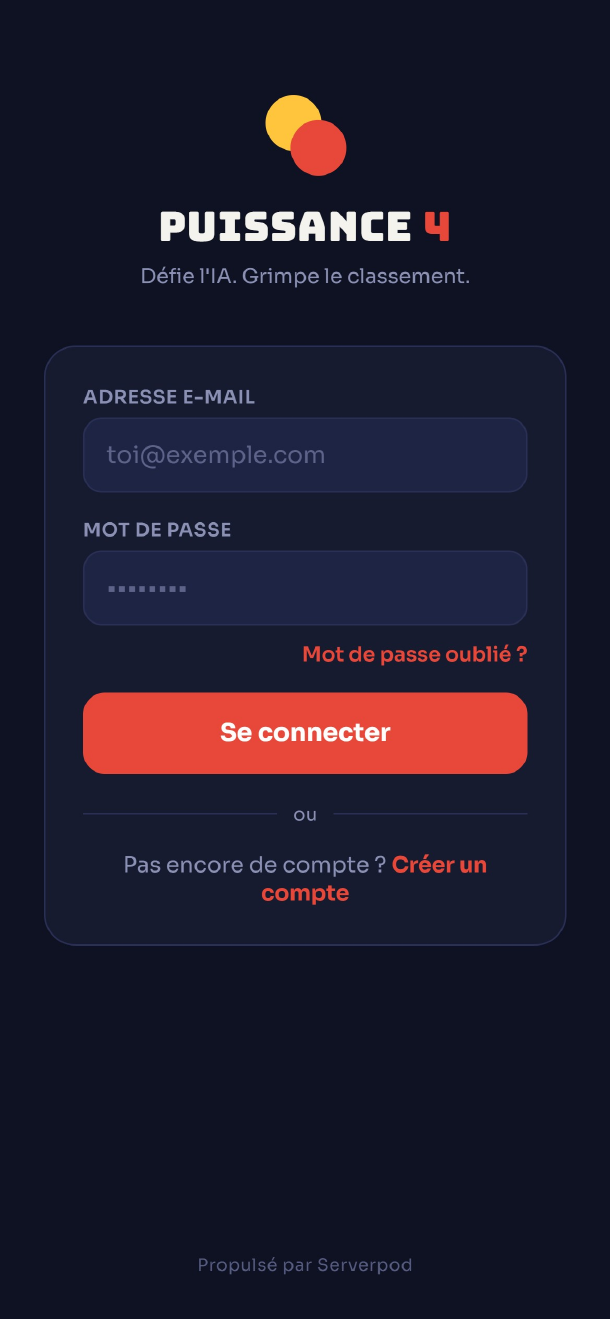
\includegraphics[height=6.5cm]{figures/maquette-1.png}\\[2pt]
\footnotesize (a) Connexion
\end{minipage}
\hfill
\begin{minipage}{0.48\textwidth}
\centering
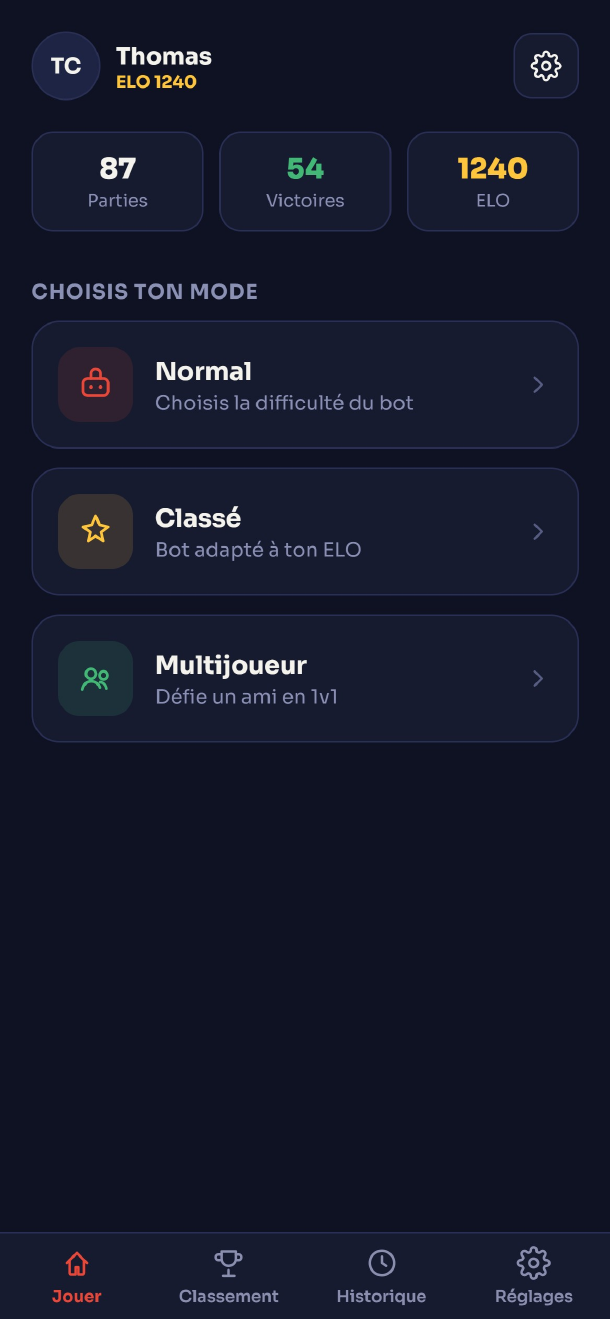
\includegraphics[height=6.5cm]{figures/maquette-2.png}\\[2pt]
\footnotesize (b) Accueil (Jouer)
\end{minipage}

\vspace{5mm}

\begin{minipage}{0.48\textwidth}
\centering
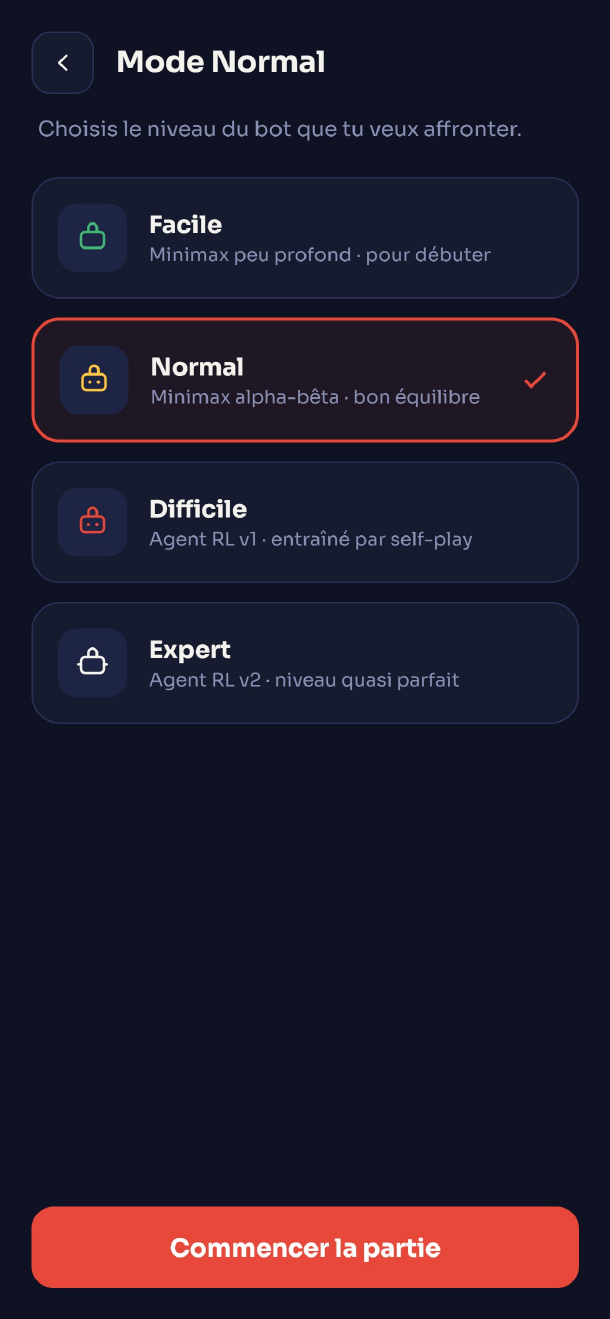
\includegraphics[height=6.5cm]{figures/maquette-3.png}\\[2pt]
\footnotesize (c) Mode Normal --- choix de la difficulté
\end{minipage}
\hfill
\begin{minipage}{0.48\textwidth}
\centering
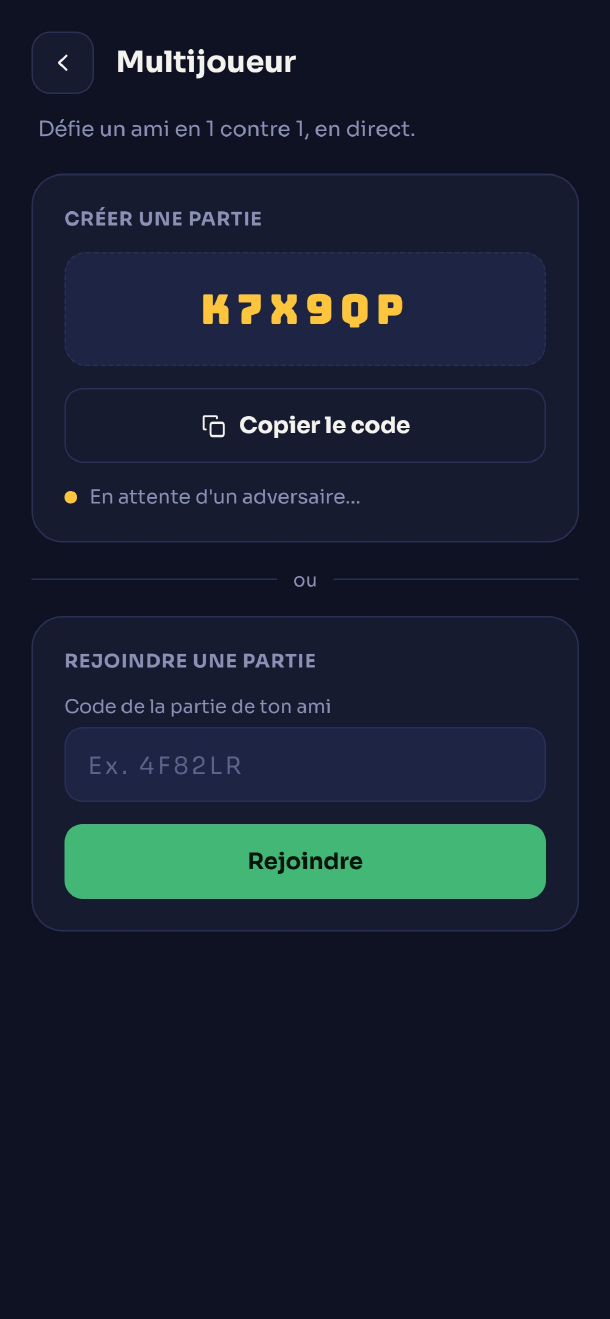
\includegraphics[height=6.5cm]{figures/maquette-4.png}\\[2pt]
\footnotesize (d) Multijoueur en ligne
\end{minipage}
\caption{Maquettes --- écrans hors-jeu (1/2)}
\label{fig:maquettes1}
\end{figure}

\begin{figure}[H]
\centering
\begin{minipage}{0.48\textwidth}
\centering
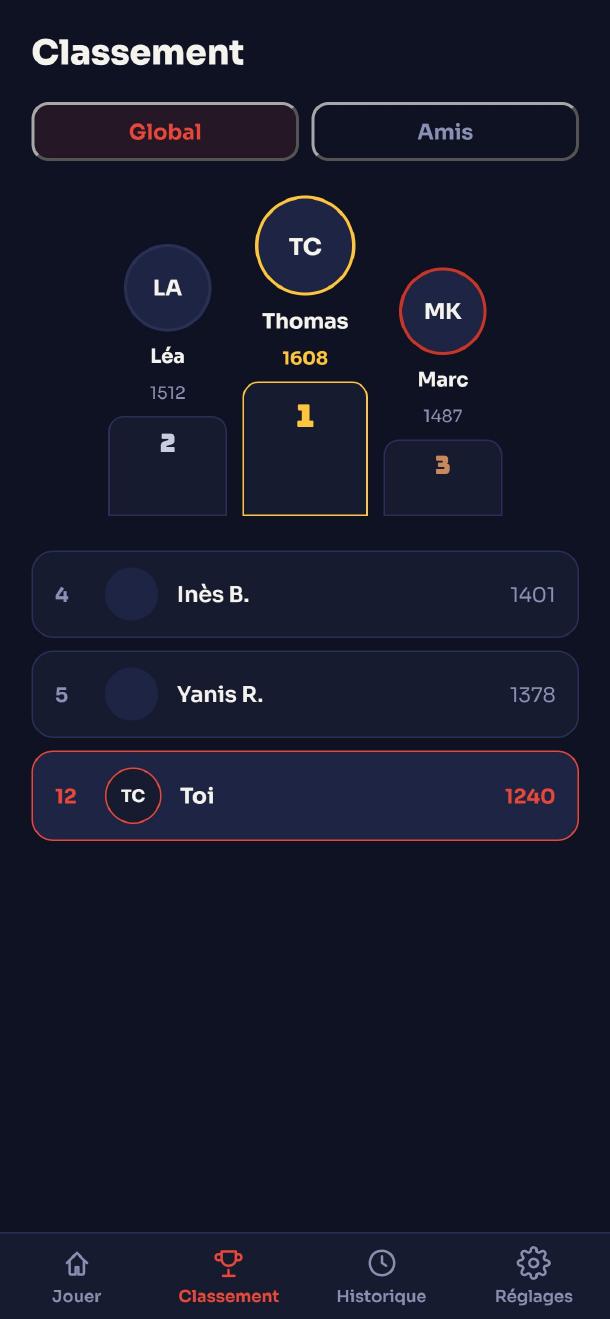
\includegraphics[height=6.5cm]{figures/maquette-5.png}\\[2pt]
\footnotesize (e) Classement
\end{minipage}
\hfill
\begin{minipage}{0.48\textwidth}
\centering
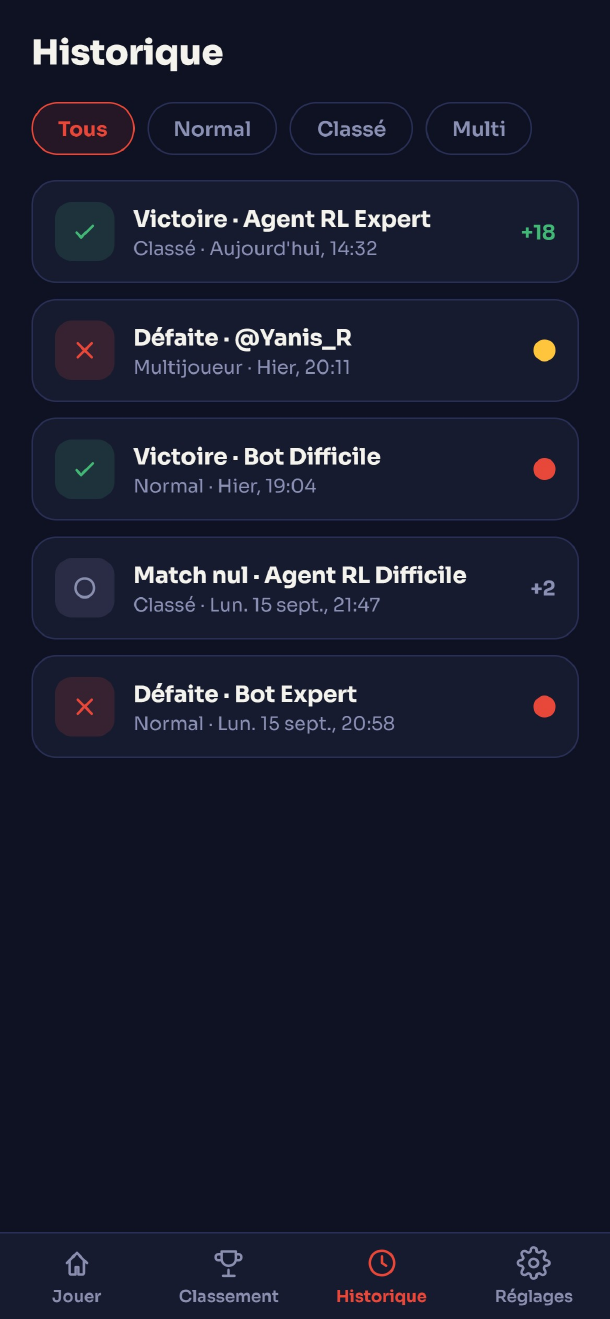
\includegraphics[height=6.5cm]{figures/maquette-6.png}\\[2pt]
\footnotesize (f) Historique des parties
\end{minipage}

\vspace{5mm}

\begin{minipage}{0.48\textwidth}
\centering
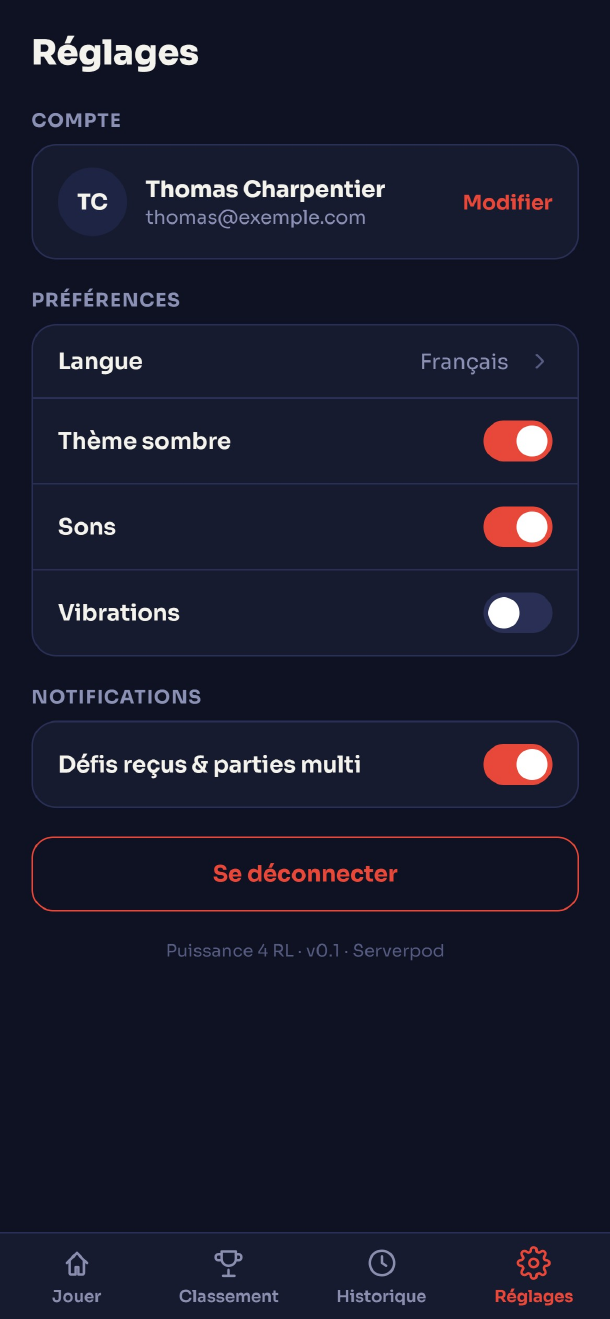
\includegraphics[height=6.5cm]{figures/maquette-7.png}\\[2pt]
\footnotesize (g) Réglages
\end{minipage}
\hfill
\begin{minipage}{0.48\textwidth}
\centering
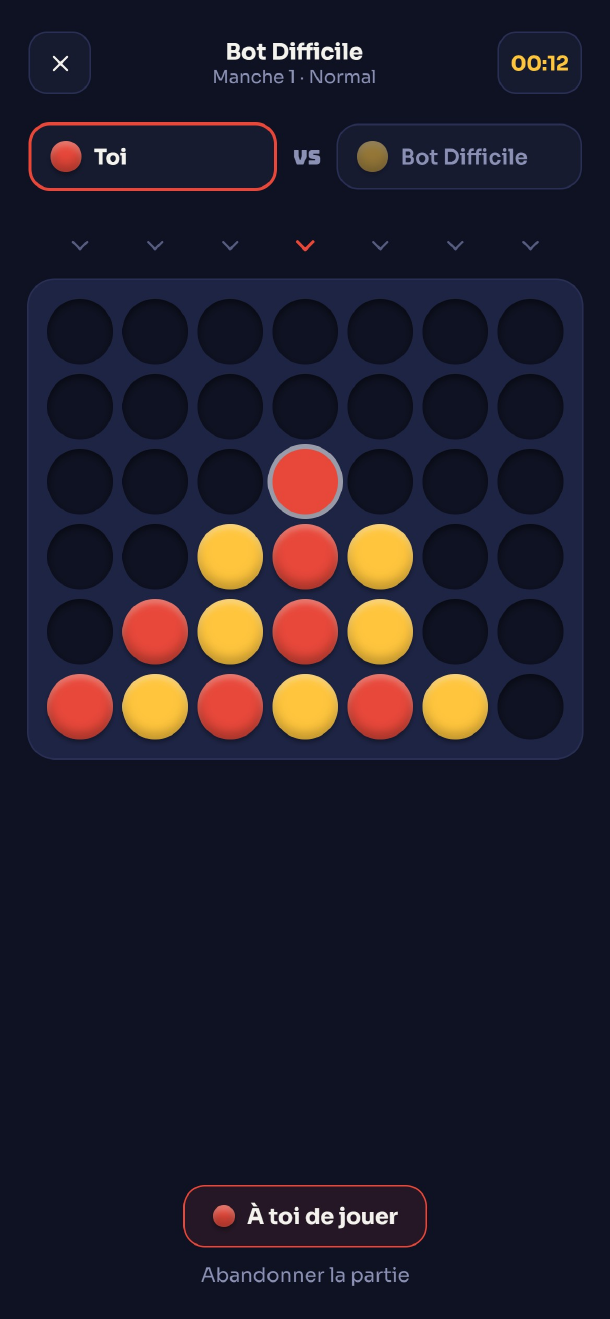
\includegraphics[height=6.5cm]{figures/maquette-8.png}\\[2pt]
\footnotesize (h) Écran de jeu
\end{minipage}
\caption{Maquettes --- écrans hors-jeu et jeu (2/2)}
\label{fig:maquettes2}
\end{figure}

\textit{Note : ces maquettes montrent 4 niveaux de bot (Facile / Normal / Difficile /
Expert, mélangeant minimax et RL) à titre d'illustration ; le choix retenu pour ce
projet est de 3 niveaux, tous basés sur des modèles RL (cf. section~4.3), les
niveaux de l'écran devront être ajustés en conséquence lors de l'implémentation.}

\section{Répartition des tâches}

\subsection{Personne A --- Firebase, UX hors-jeu \& Infra}
\begin{itemize}[leftmargin=1.5em]
  \item UI des écrans hors-jeu (accueil, login, profil, leaderboard, paramètres,
        navigation, l10n).
  \item Login/inscription (Firebase Auth) et intégration du pont vers le compte de
        jeu Serverpod.
  \item Photo de profil (caméra + stockage Serverpod).
  \item Leaderboard et écran d'historique (consommation des endpoints Serverpod).
  \item Détection ``posé à plat'' $\rightarrow$ mise en pause automatique.
  \item Pipeline CI/CD (lint, tests, build APK, déploiement du serveur Serverpod).
\end{itemize}

\subsection{Personne B --- Backend Serverpod, Jeu \& IA}
\begin{itemize}[leftmargin=1.5em]
  \item Setup initial du repo Flutter et du projet Serverpod (endpoints, schéma
        PostgreSQL).
  \item UI de l'écran de jeu et logique du Puissance 4 (règles, victoire/égalité).
  \item Les 3 sous-modes : Normal, Ligue/Classé, Multijoueur en ligne.
  \item Reset par secousse (mode Normal uniquement).
  \item Entraînement RL sur Colab (3 niveaux), export, inférence locale, endpoint de
        distribution des modèles.
  \item Système Elo (calcul et persistance Serverpod).
  \item Enregistrement des résultats de partie (historique).
\end{itemize}

\section{Lien avec les critères du cours}

\begin{itemize}[leftmargin=1.5em]
  \item \textbf{Context-aware / capteurs} : caméra (photo de profil) + accéléromètre
        (reset par secousse, détection ``posé à plat'' $\rightarrow$ pause
        automatique) --- au moins deux capteurs, dont un comportement réellement
        adaptatif au contexte physique.
  \item \textbf{Originalité} : modèle de RL entraîné hors-app et exécuté en
        inférence embarquée (edge AI), matchmaking Elo adaptatif, backend full-stack
        Dart (Serverpod) gérant multijoueur temps réel et distribution de modèles.
  \item \textbf{l10n} : application prévue en français et anglais au minimum.
\end{itemize}

\section{Points ouverts et risques}
\label{sec:risques}

\begin{itemize}[leftmargin=1.5em]
  \item \textbf{Pont d'authentification} Firebase $\rightarrow$ Serverpod : à
        concevoir et tester tôt, c'est un point critique d'intégration.
  \item \textbf{Confiance côté client en mode Classé} : un résultat de partie contre
        le bot est déclaré par le client ; risque de triche assumé pour ce projet.
  \item \textbf{Cohérence des niveaux de bot} entre le cahier des charges (3 niveaux
        RL) et les maquettes existantes (4 niveaux, minimax + RL) à clarifier avant
        implémentation de l'écran de sélection de difficulté.
  \item \textbf{Protocole temps réel} du multijoueur (reconnexion, abandon/timeout
        d'un joueur, validité du code de partie) à spécifier plus finement lors du
        développement du module Serverpod correspondant.
\end{itemize}

\end{document}
